% Golden Spiral can be approximated with Golden ratio or Fibonacci sequence.
% Golden Ratio: a+b/a = a/b

\documentclass{beamer}
\usepackage[utf8]{inputenc}
\usepackage[T1]{fontenc}

\usetheme{Cuerna}
\usecolortheme{default}
% default, bluesimplex, lettuce, brick

\title{AML-RL Final Project}
\author{Shayan Amani}

\date{fall 2018}
\institute{Department of Computer Science, University of New Hampshire}

\begin{document}

\begin{frame}
    \titlepage
\end{frame}

\begin{frame}{Methodology}
\textbf{Deep Q-Network}

Why?
\begin{itemize}
    \item Applying a non-linear approximator such as neural networks seems reasonable to reveal unseen relations between among data samples.
    \item Inquisitiveness 
    \item Q-learning performed well in the literature.
\end{itemize} \\\\
In that sense: \\
\centering  Q-learning + neural networks $\rightarrow$ DQN
\end{frame}



\begin{frame}{Ideas}

  This approach take advantage of two key ideas:
  \begin{enumerate}
      \item Experience Replay: randomized sample drawing to breaks correlations between consecutive observations.
      \item Frequent Q updates: adjusts action-values (Q) iteratively.
  \end{enumerate}
\end{frame}

\begin{frame}{Algorithm}
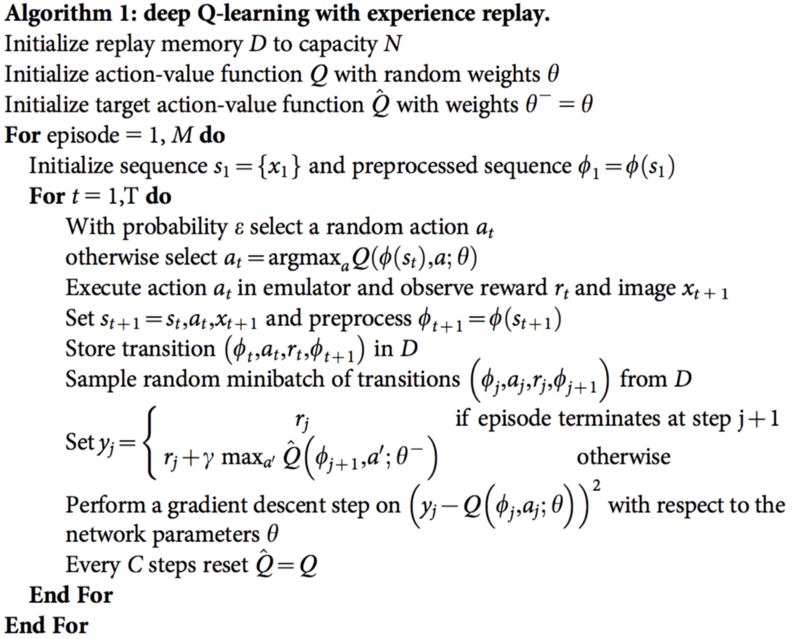
\includegraphics[scale=0.3]{alg-dqn.png}
    
\end{frame}

\begin{frame}{Architecture}
    The neural network:
    \begin{itemize}
        \item 3 dense layers
        \item ReLU activation function
        \item features fed in as inputs
        \item 2 action-values (Q values) as output
    \end{itemize}
    
\end{frame}

\begin{frame}{Training}

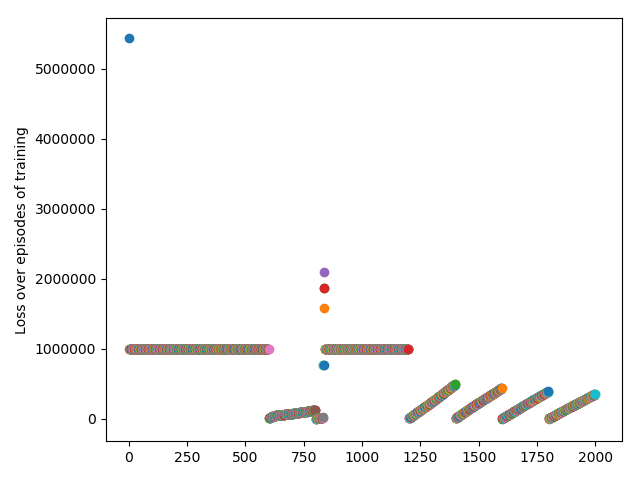
\includegraphics[scale=0.35]{myplot.png}

    
\end{frame}

  
\begin{frame}{Other Proposed Techniques}
    \item \textbf{$\epsilon$-greedy exploration}: batch learning vs online learning
    \item \textbf{reward clipping}: doesn't remarkably affect the Q values.
\end{frame}
  
  
\begin{frame}{Applied Techniques}
Random batch sampling from the memory of samples to break correlation between consecutive samples (i.e. consecutive years).

\end{frame}

	%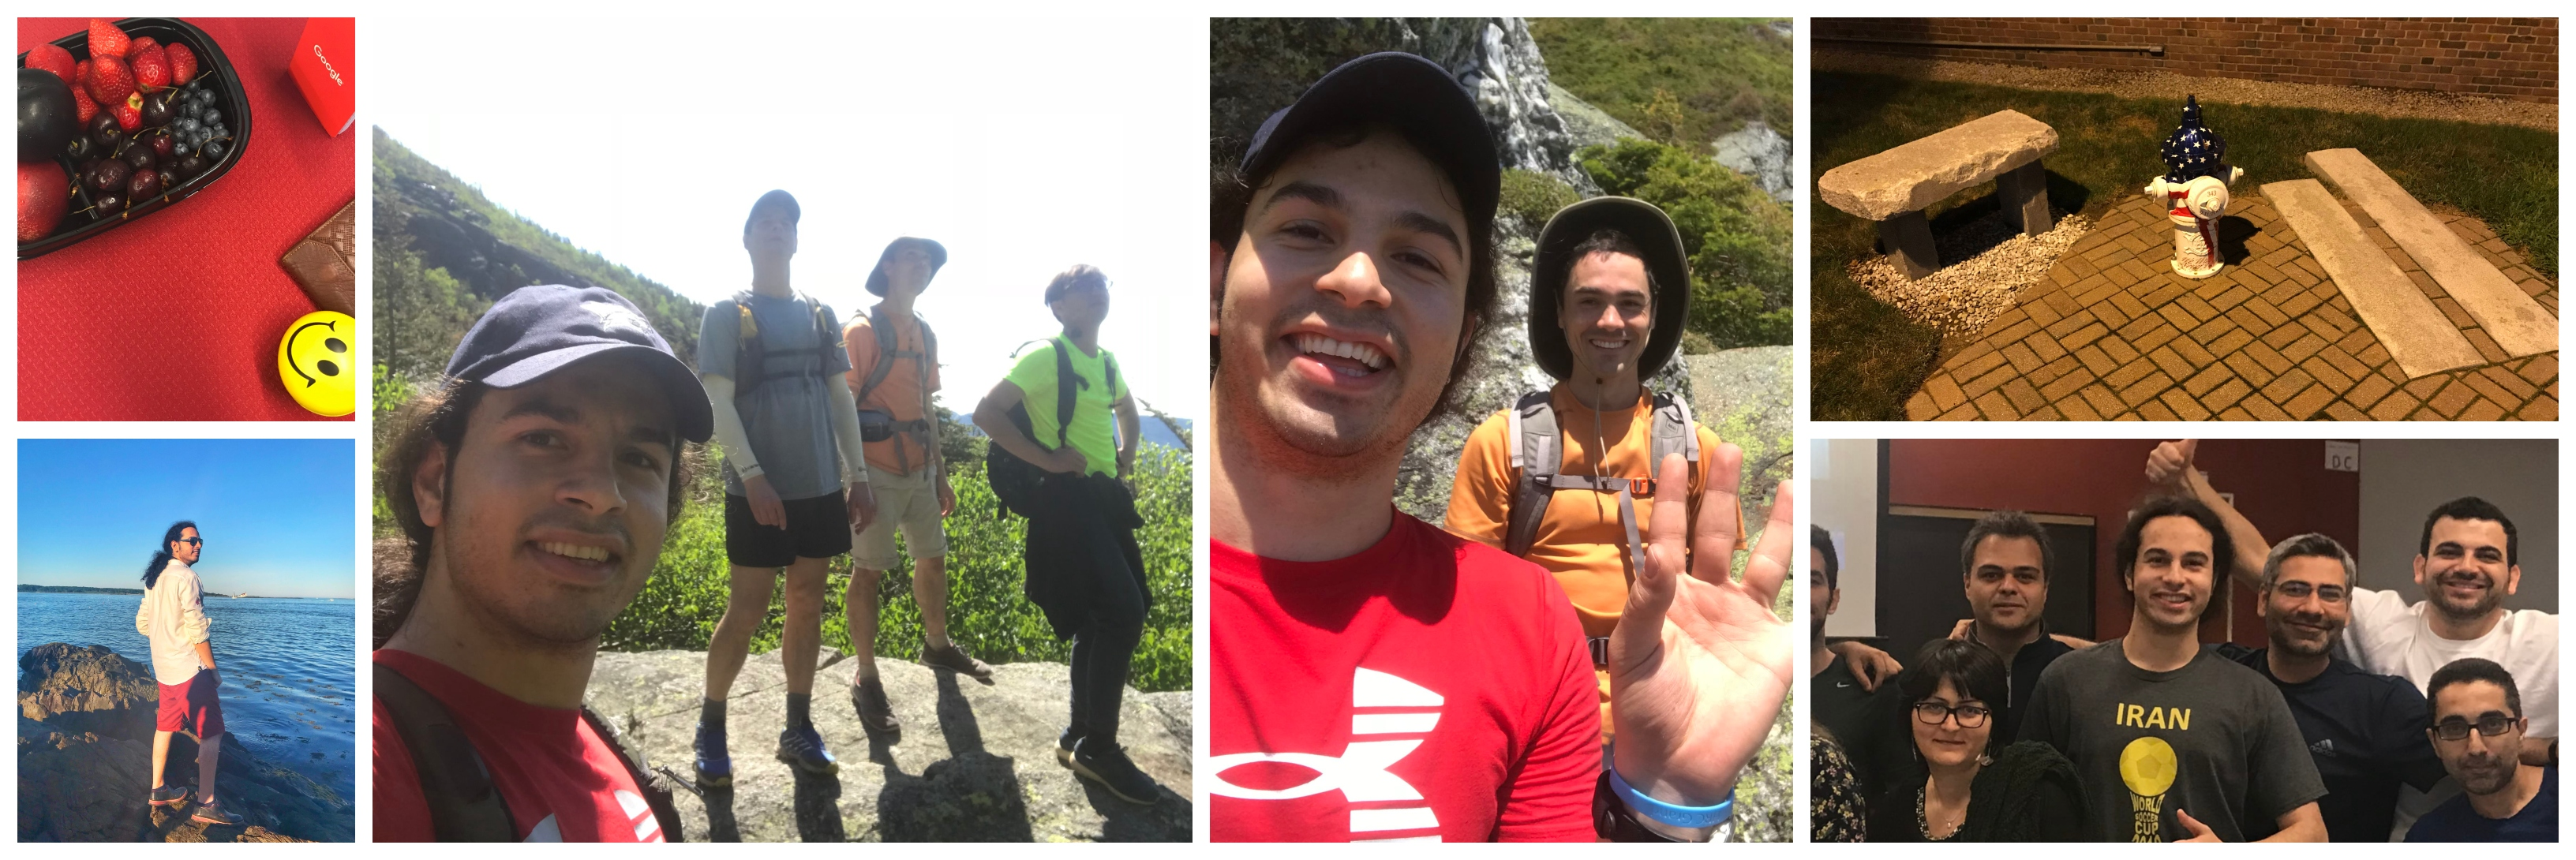
\includegraphics[scale=0.45]{img.jpg}
	
% \begin{frame}{To-Do}

% \begin{itemize}
%  \item add more layers
%  \item describe ExpRep in slides
%  \item PCA
%  \item reward clipping
%  \item other variation of DQN
%  \item get rid of game over
%  \item model training for 500 epochs
%  \item q learning implementation vs qnet
%  \item pytorch imp
% \end{itemize}
    
% \end{frame}

\begin{frame}{Future Steps}
\begin{itemize}
    \item Applying Double Q-Networks and other acclaimed working variation of the configuration. 
    \item Take a deeper look at the features interactions
    \item Tuning hyper-parameters like learning rate in case of bigger set of samples.
\end{itemize}
\end{frame}


\begin{frame}{Acknowledgment}
\begin{itemize}
    \item UC Berkley’s course on deep reinforcement learning
    \item Algorithm adapted from \href{http://artint.info/html/ArtInt_265.html}{\textit{Artificial Intelligence: Foundations of Computational Agents, second edition, Cambridge University Press 2017}}
\end{itemize}
\end{frame}


\end{document}




%     \section{Questions}
% \begin{itemize}
%     \item 2000 samples for 10 times of 200 years. What kind of times?
%     \item What are states? How many?
% \end{itemize}

% \section{Definition}
% We have 2000 samples for 200 years. In terms of games, this is like a already played game and we have the history of the gameplay.

% \subsection{State}
% each row

% \subsection{Action}
% 2 actions: 0 and 10.
% $\epsilon$-greedy exploration is not applied, because we have no control over agent.

% \subsection{Reward}
% A summation according to it's definition.



% We can use either On-Policy or Off-Policy methods. From the given samples it could be simply inferred that a model-free algorithm is needed and the reason is that the problem doesn't provide the transition probabilities.
